\chapter{Simulation Studies}
\label{chap:Simulation}
The previous chapter compared the static and dynamic schedules in terms of the expected cost of each schedule. We found for $15$ customers, the dynamic schedule is about $5 - 10 \%$ better than the static schedule depending on the value of $\gamma$. However, this does not provide any information about the other properties of each schedule. For example, one of the schedules could have a greater variability in customer waiting times.

To understand each schedule more fully, we use a simulation study. We simulated a million runs and measured the performance of both schedules on each run. Each run involved simulating the service times of the $15$ customers assuming $\mu = 1$. All the simulations were completed assuming $\gamma = 0.5$.

\section{Schedule Cost}
The mean costs of the static and dynamic schedules were $15.05$ and $13.55$ respectively. As expected, these mean costs closely match the expected costs of the schedules. Figure~\ref{fig:Two_Cost} plots the histograms of the costs of the static and dynamic schedules for each run of the simulation.
\begin{figure}[htb]
	\centering
	\begin{subfigure}[t]{0.45\textwidth}
		\centering
		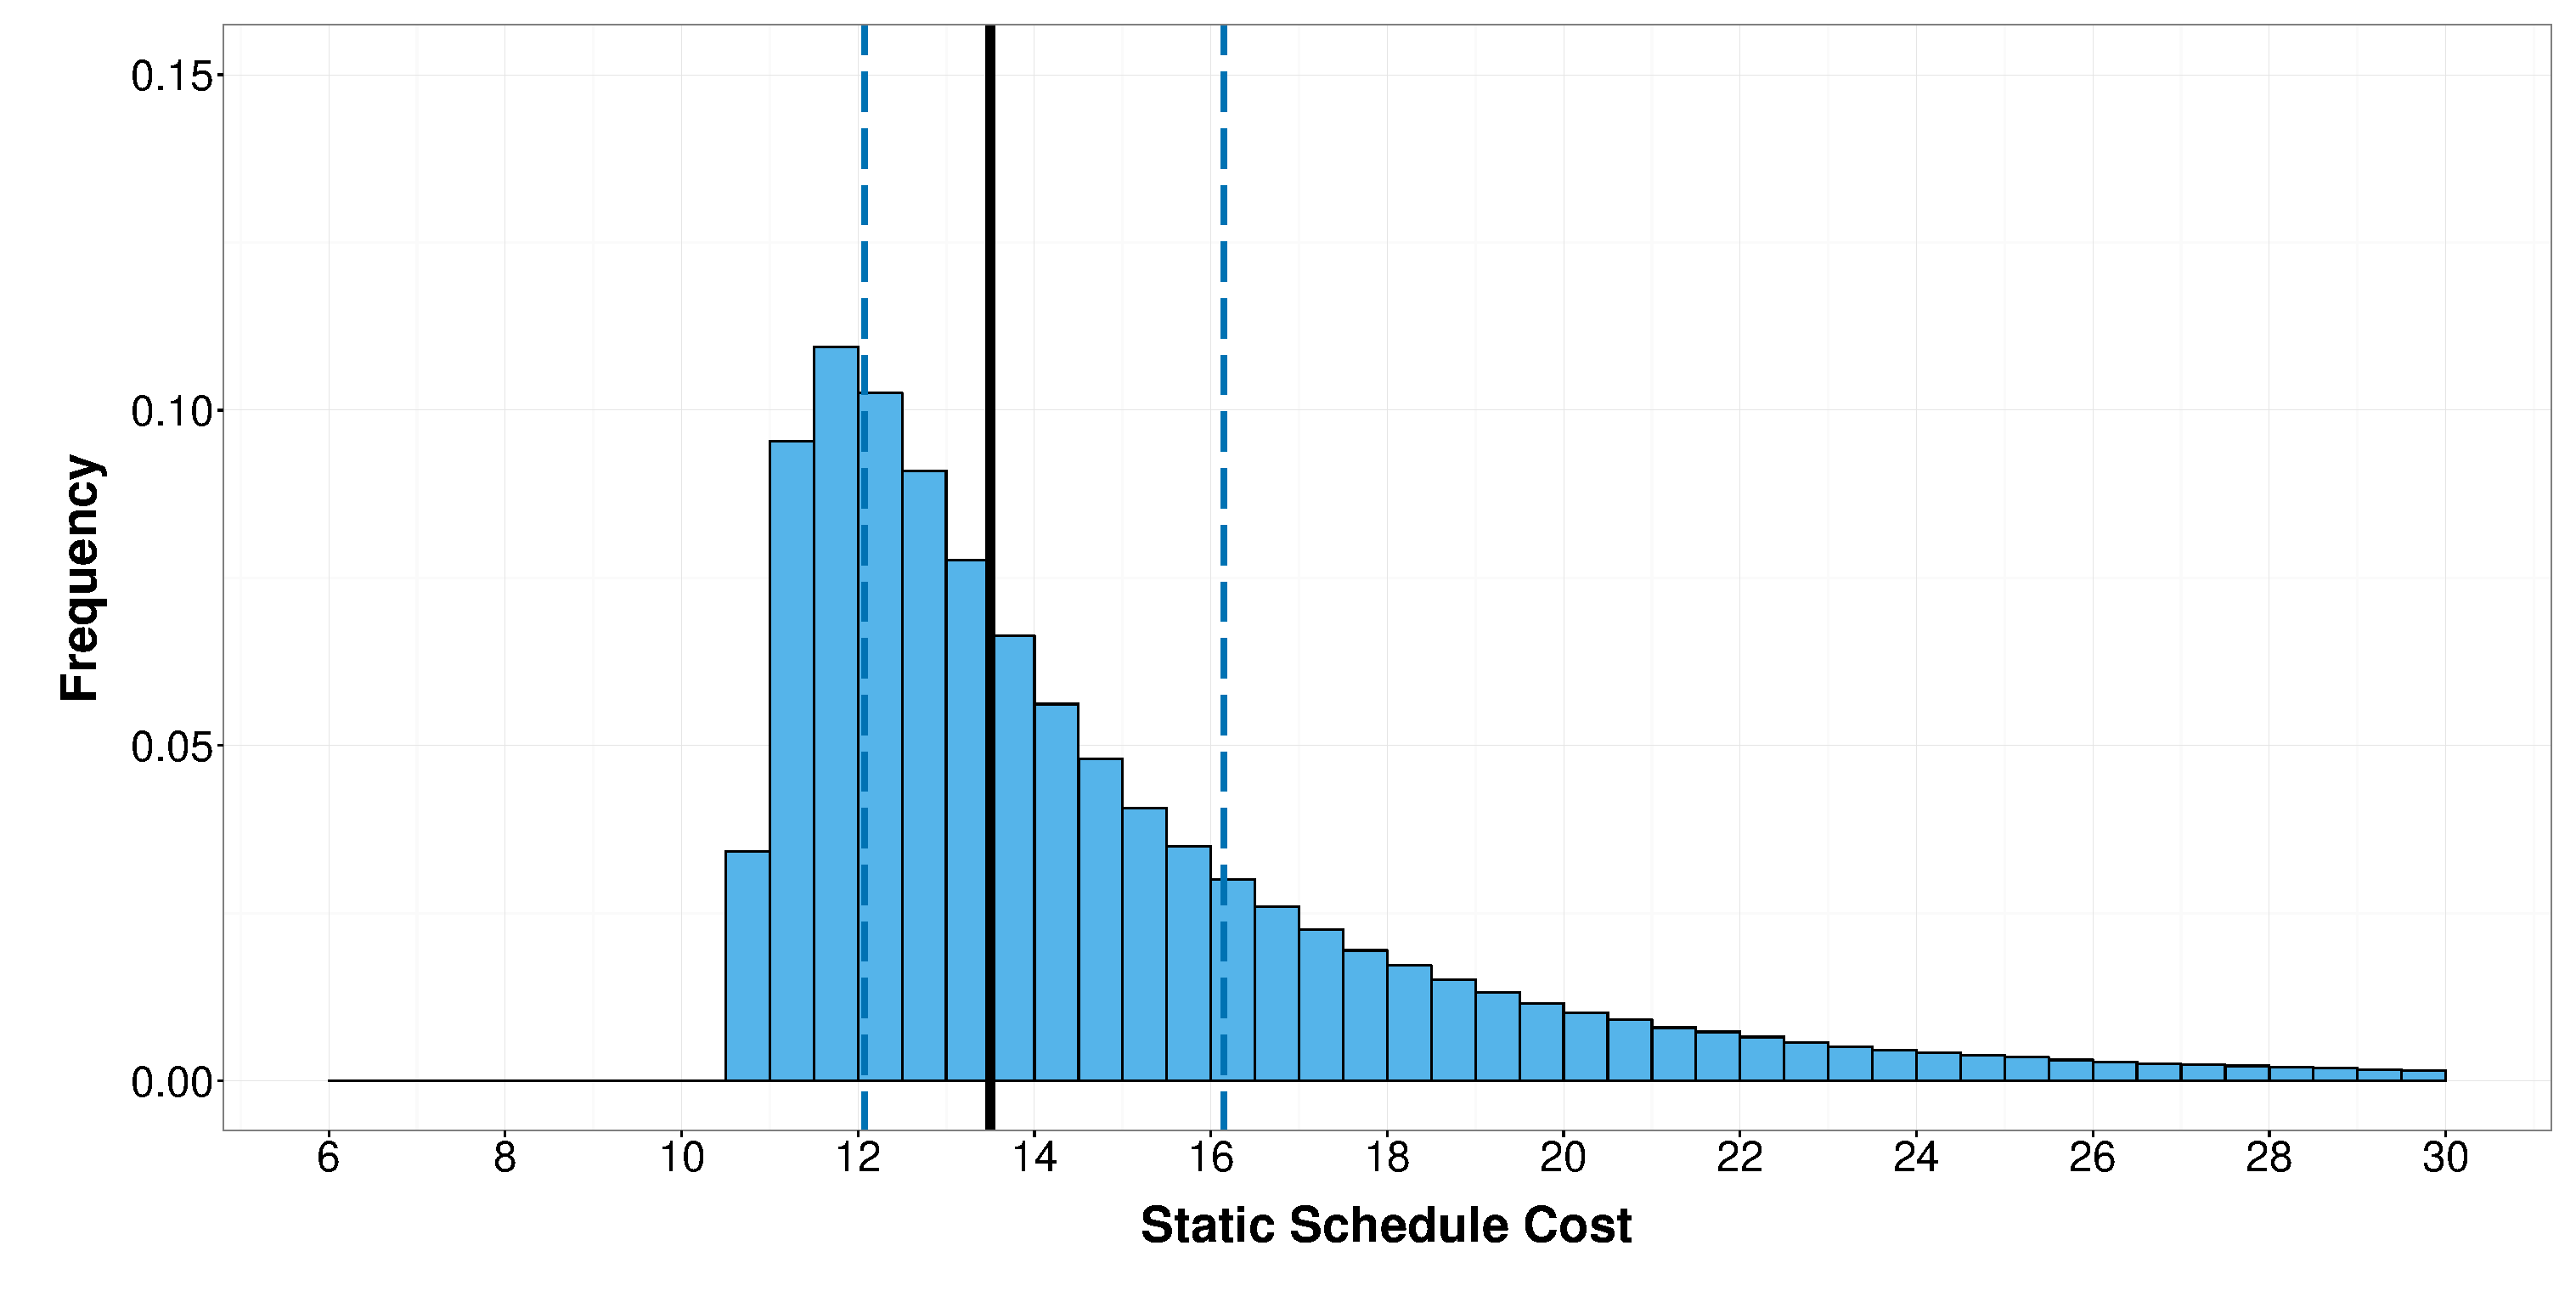
\includegraphics[width=\textwidth]{Cost_Hist_Static.eps}
		\caption{}
	\end{subfigure}
	\begin{subfigure}[t]{0.45\textwidth}
		\centering
		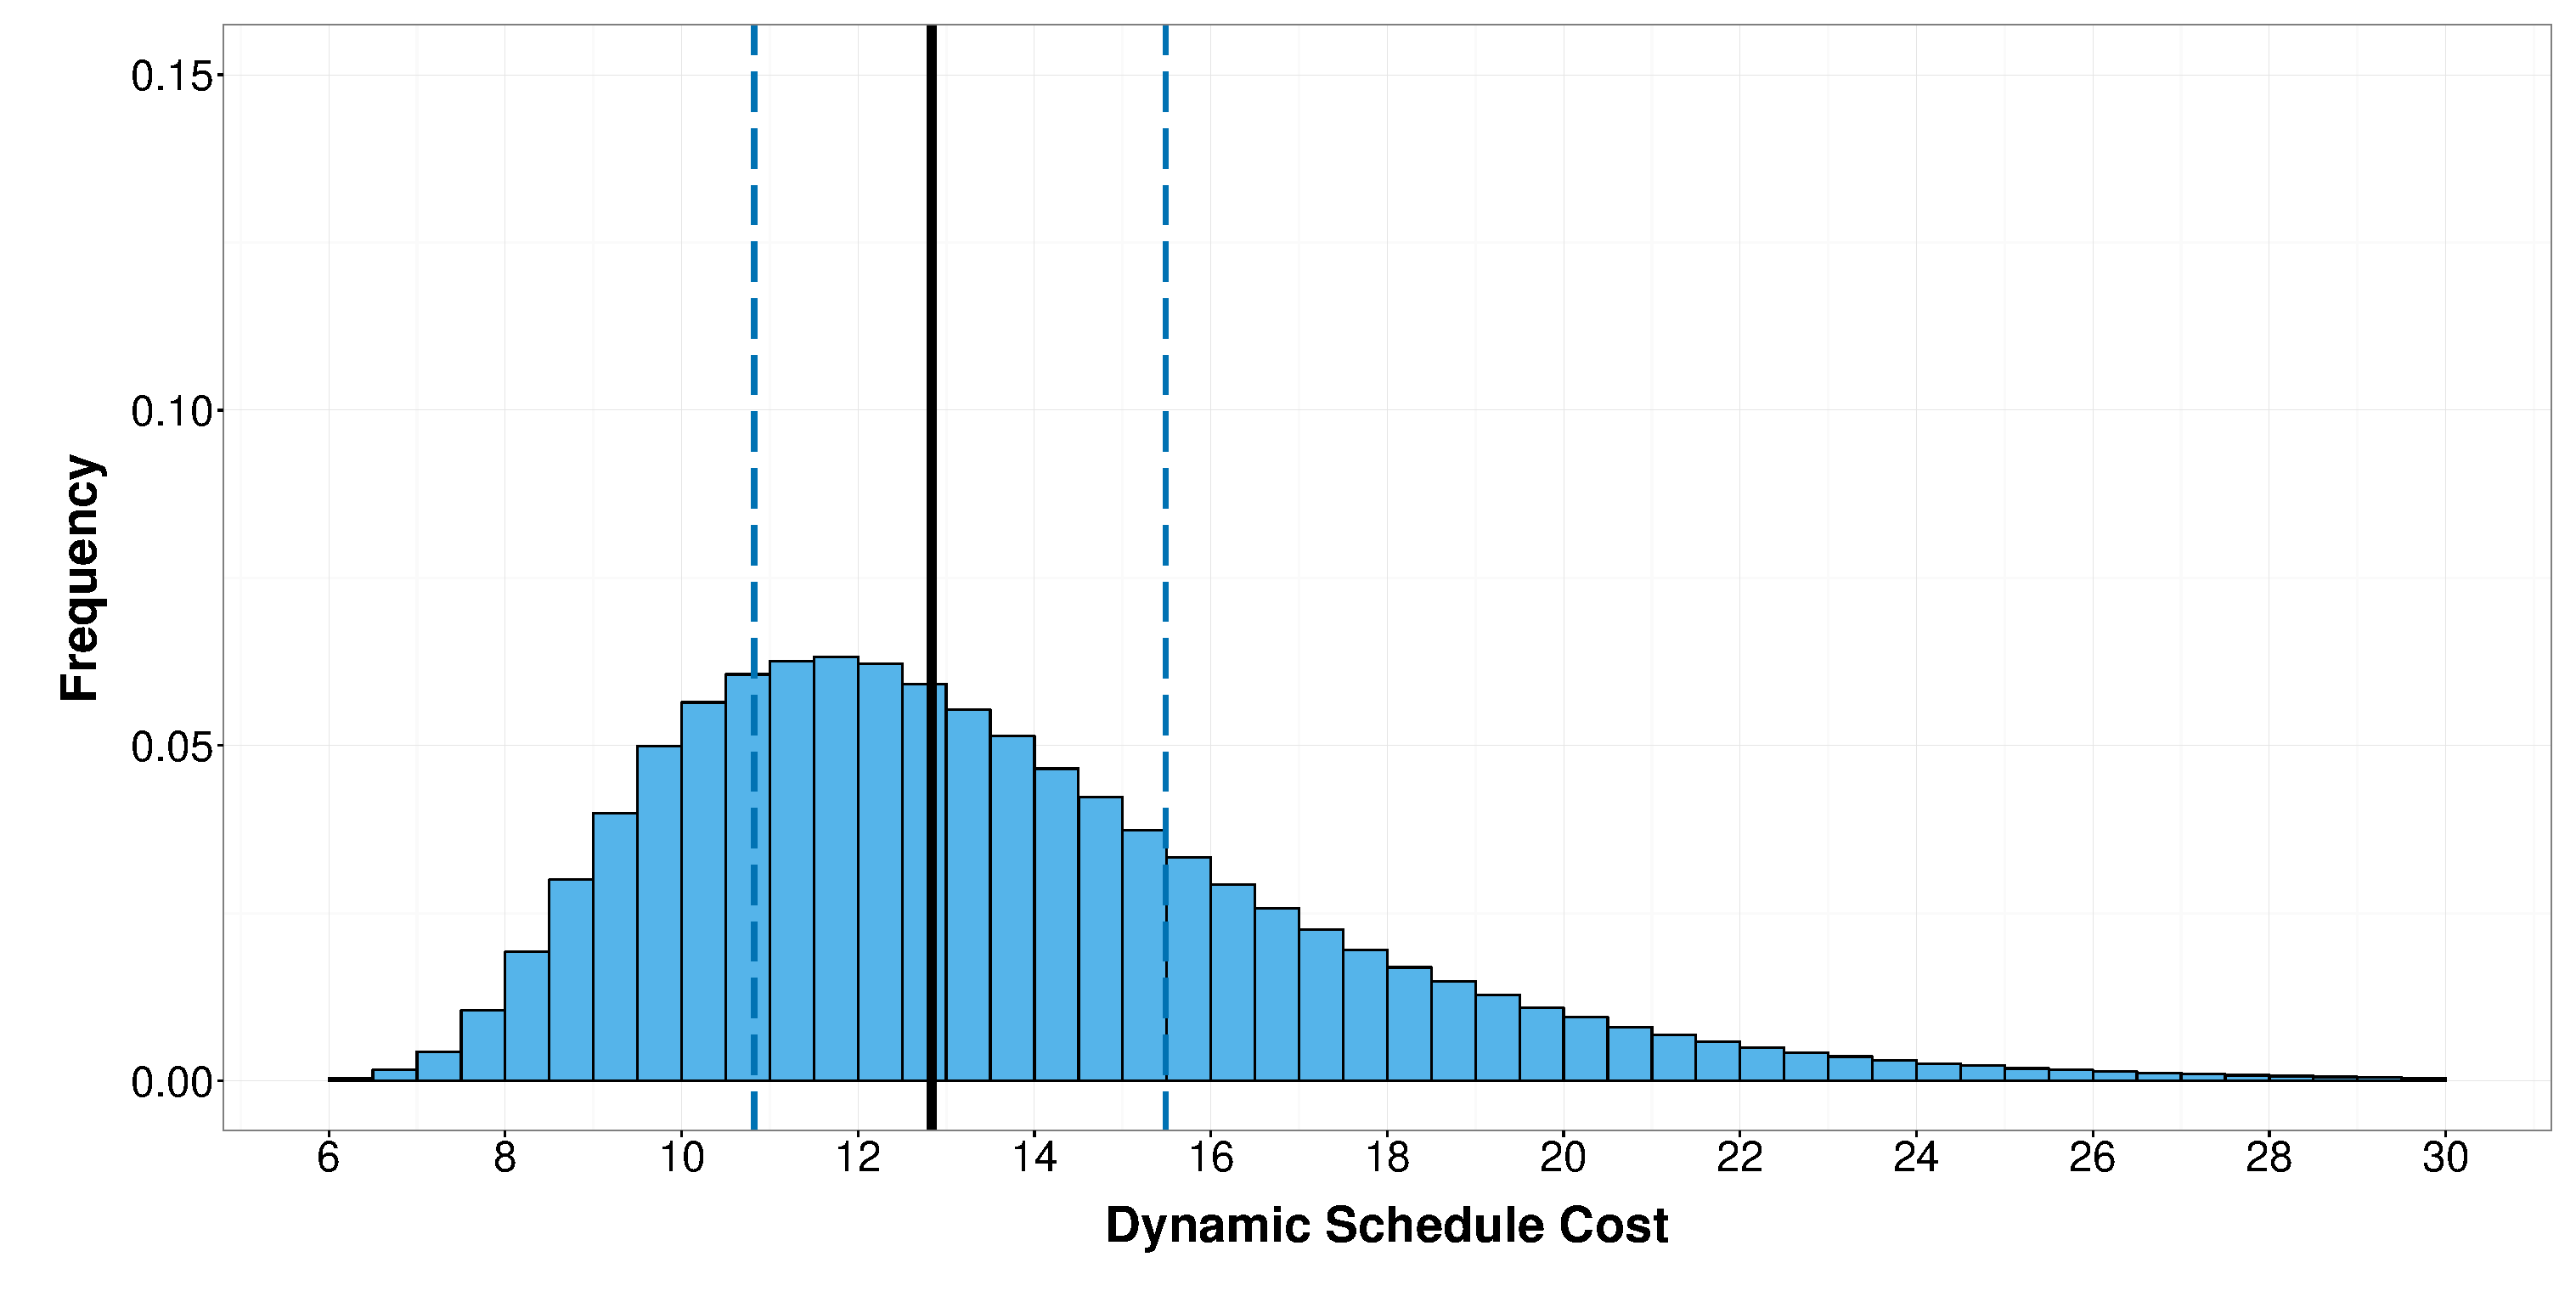
\includegraphics[width=\textwidth]{Cost_Hist_Dynamic.eps}
		\caption{}
	\end{subfigure}
	\caption{Histogram plot of the costs of the static (a) and dynamic (b) schedules for each simulation run where $\mu = 1$ and $\gamma = \frac{c_{S}}{c_{S} + c_{W}} = 0.5$. The black vertical line indicates the median and the blue dashes lines indicate the upper and lower quartiles.}
	\label{fig:Two_Cost}
\end{figure}

The distribution of the cost of the static schedule is right skewed. The peak of the distribution occurs at around 12, but the median is $13.5$. In contrast, the distribution of the dynamic schedule is more symmetric with the peak occurring closer to the median of $12.8$. The dynamic schedule is more flexible and thus less prone to runs with extremely high cost.

Figure~\ref{fig:Diff_Cost} plots the histogram of the difference in costs between the two schedules. This is a plot of the cost of the static schedule minus the cost of the dynamic schedule for the same run.
\begin{figure}[htb]
	\centering
	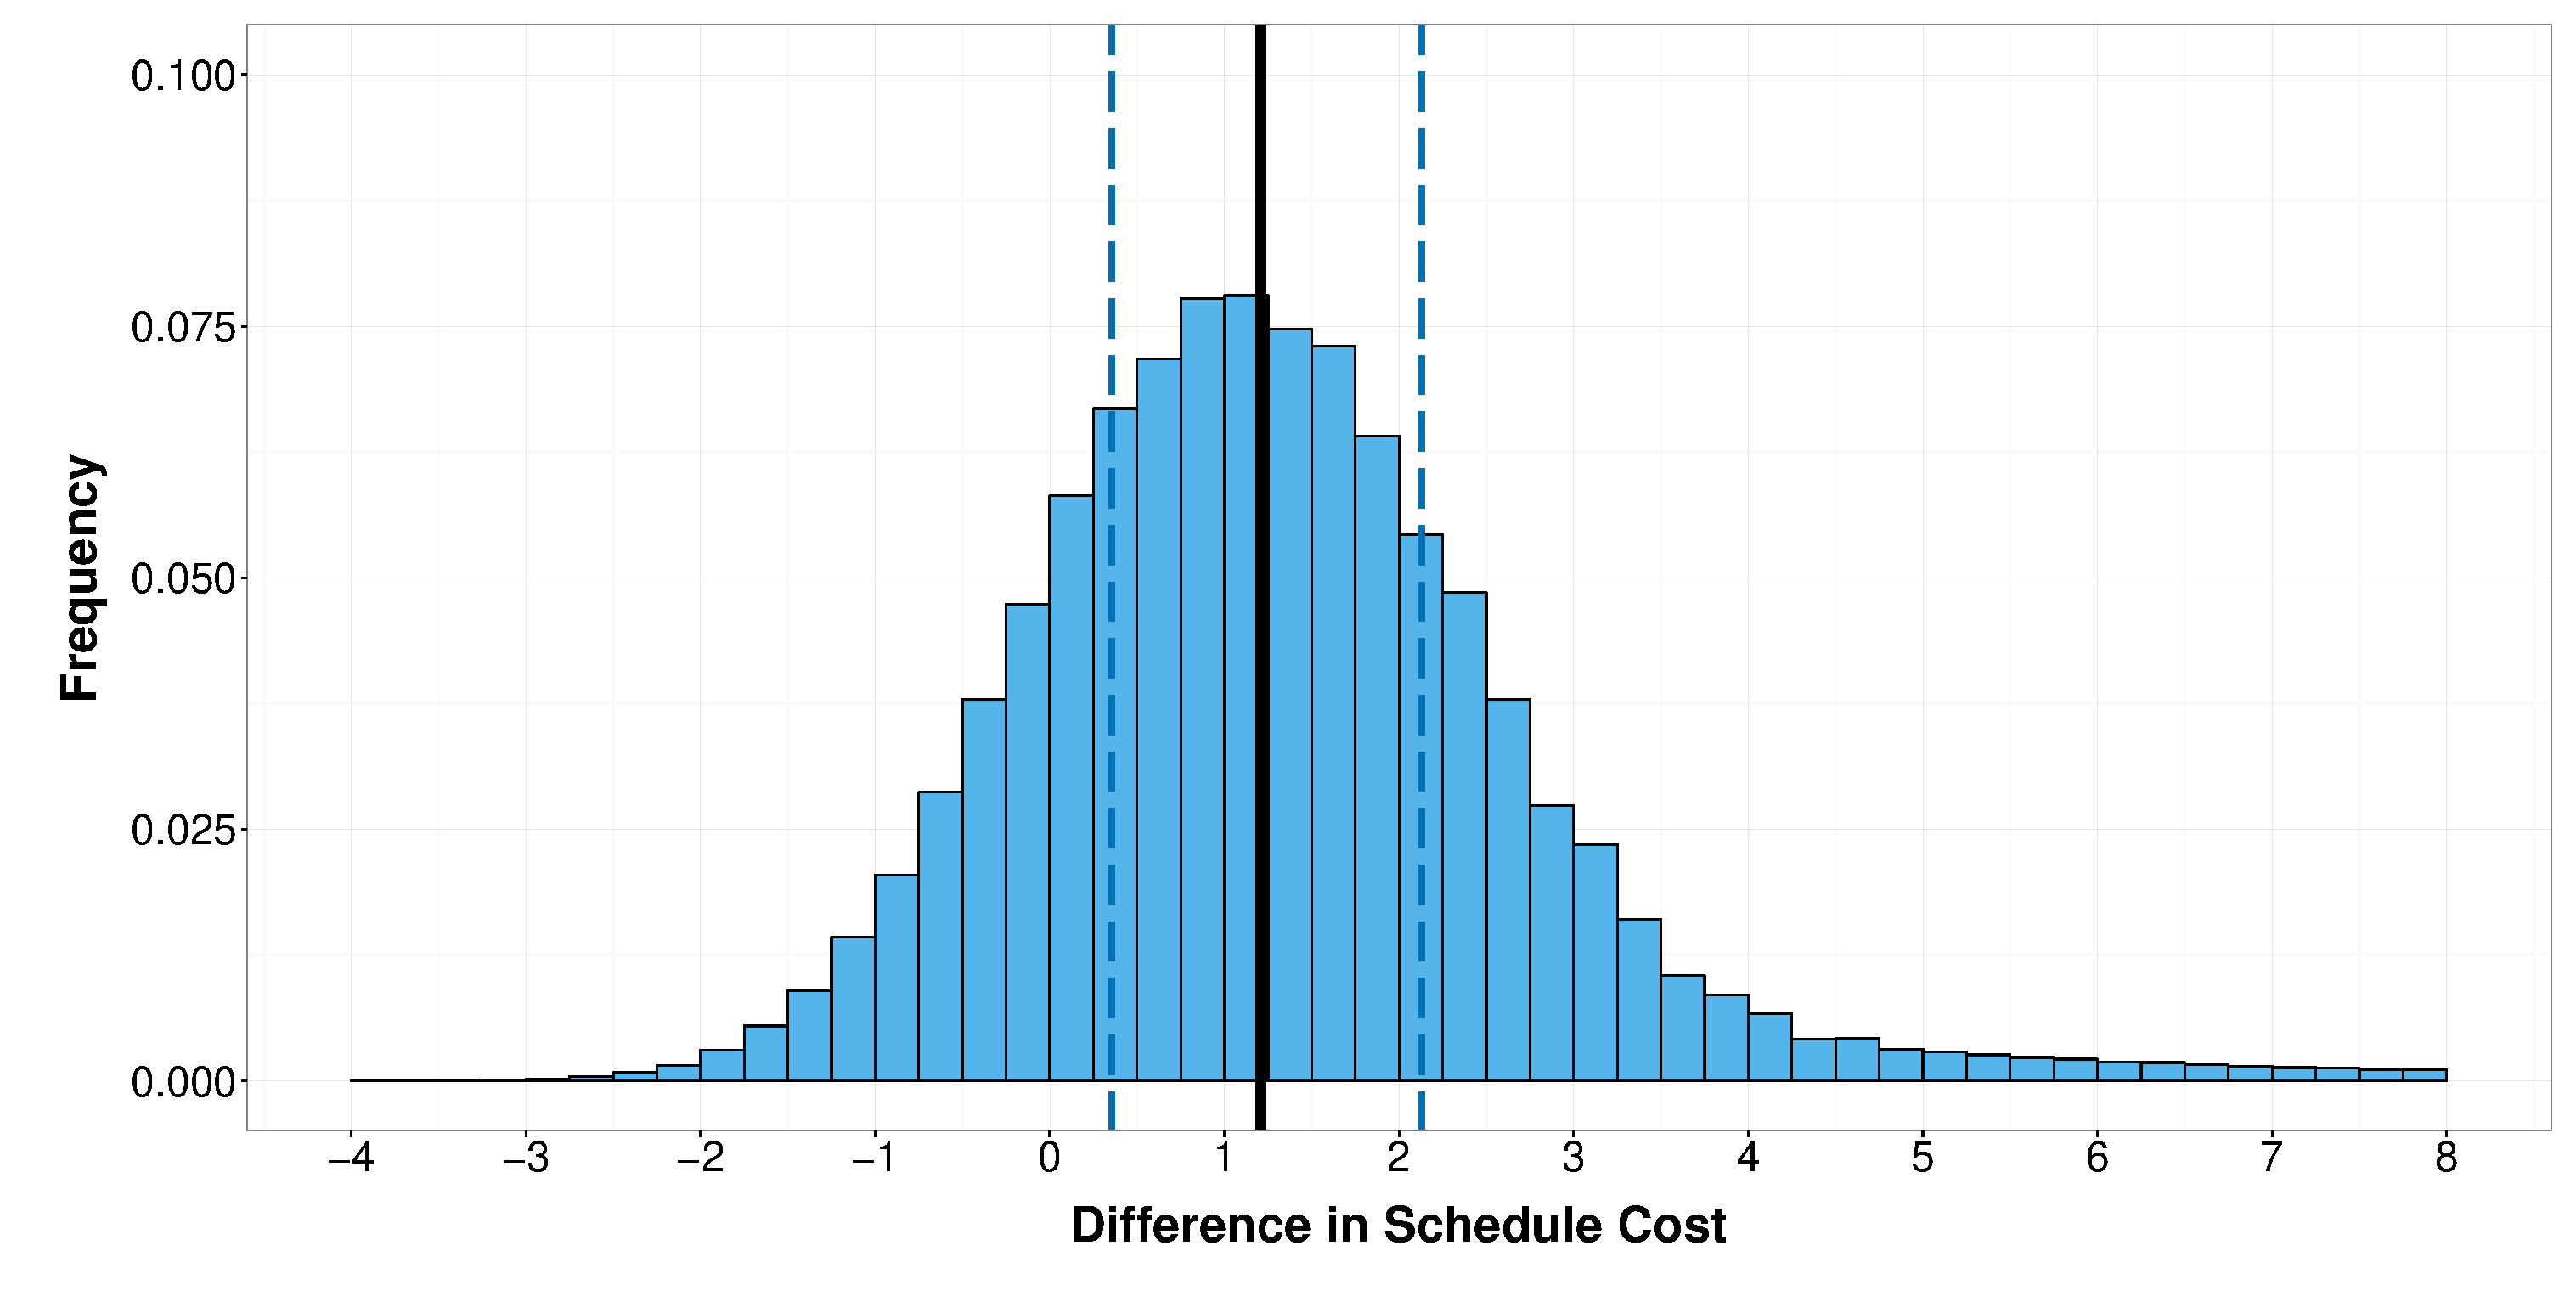
\includegraphics[width = 0.85\textwidth]{Cost_Hist_Diff.eps}
	\caption{Histogram plot of the cost of the static schedule minus the cost of the dynamic schedule for each simulation run where $\mu = 1$ and $\gamma = \frac{c_{S}}{c_{S} + c_{W}} = 0.5$. The black vertical line indicates the median and the blue dashes lines indicate the upper and lower quartiles.}
	\label{fig:Diff_Cost}
\end{figure}

While the expected cost of the static schedule is greater than the expected cost of the dynamic schedule, the static schedule outperforms the dynamic schedule for a proportion of the simulation runs. This is indicated by a negative cost difference in Figure~\ref{fig:Diff_Cost}. The $25$-th percentile of the cost difference is $0.35$. For more than $75 \%$ of runs, the static schedule has a larger cost than the dynamic schedule. The $75$-th percentile is $2.13$ (i.e., more than twice the mean service time). For a large proportion of the runs, the dynamic schedule significantly outperforms the static schedule.

\section{Customer Arrival Times}
We have observed that the dynamic schedule performs better than the static schedule both in expectation and for the majority of the simulation runs. The next step is to attempt to understand how the dynamic schedule is able to outperform the static schedule. Figure~\ref{fig:Avg_Arrival} plots the average arrival time of the $15$ customers for the two schedules.
\begin{figure}[htb]
	\centering
	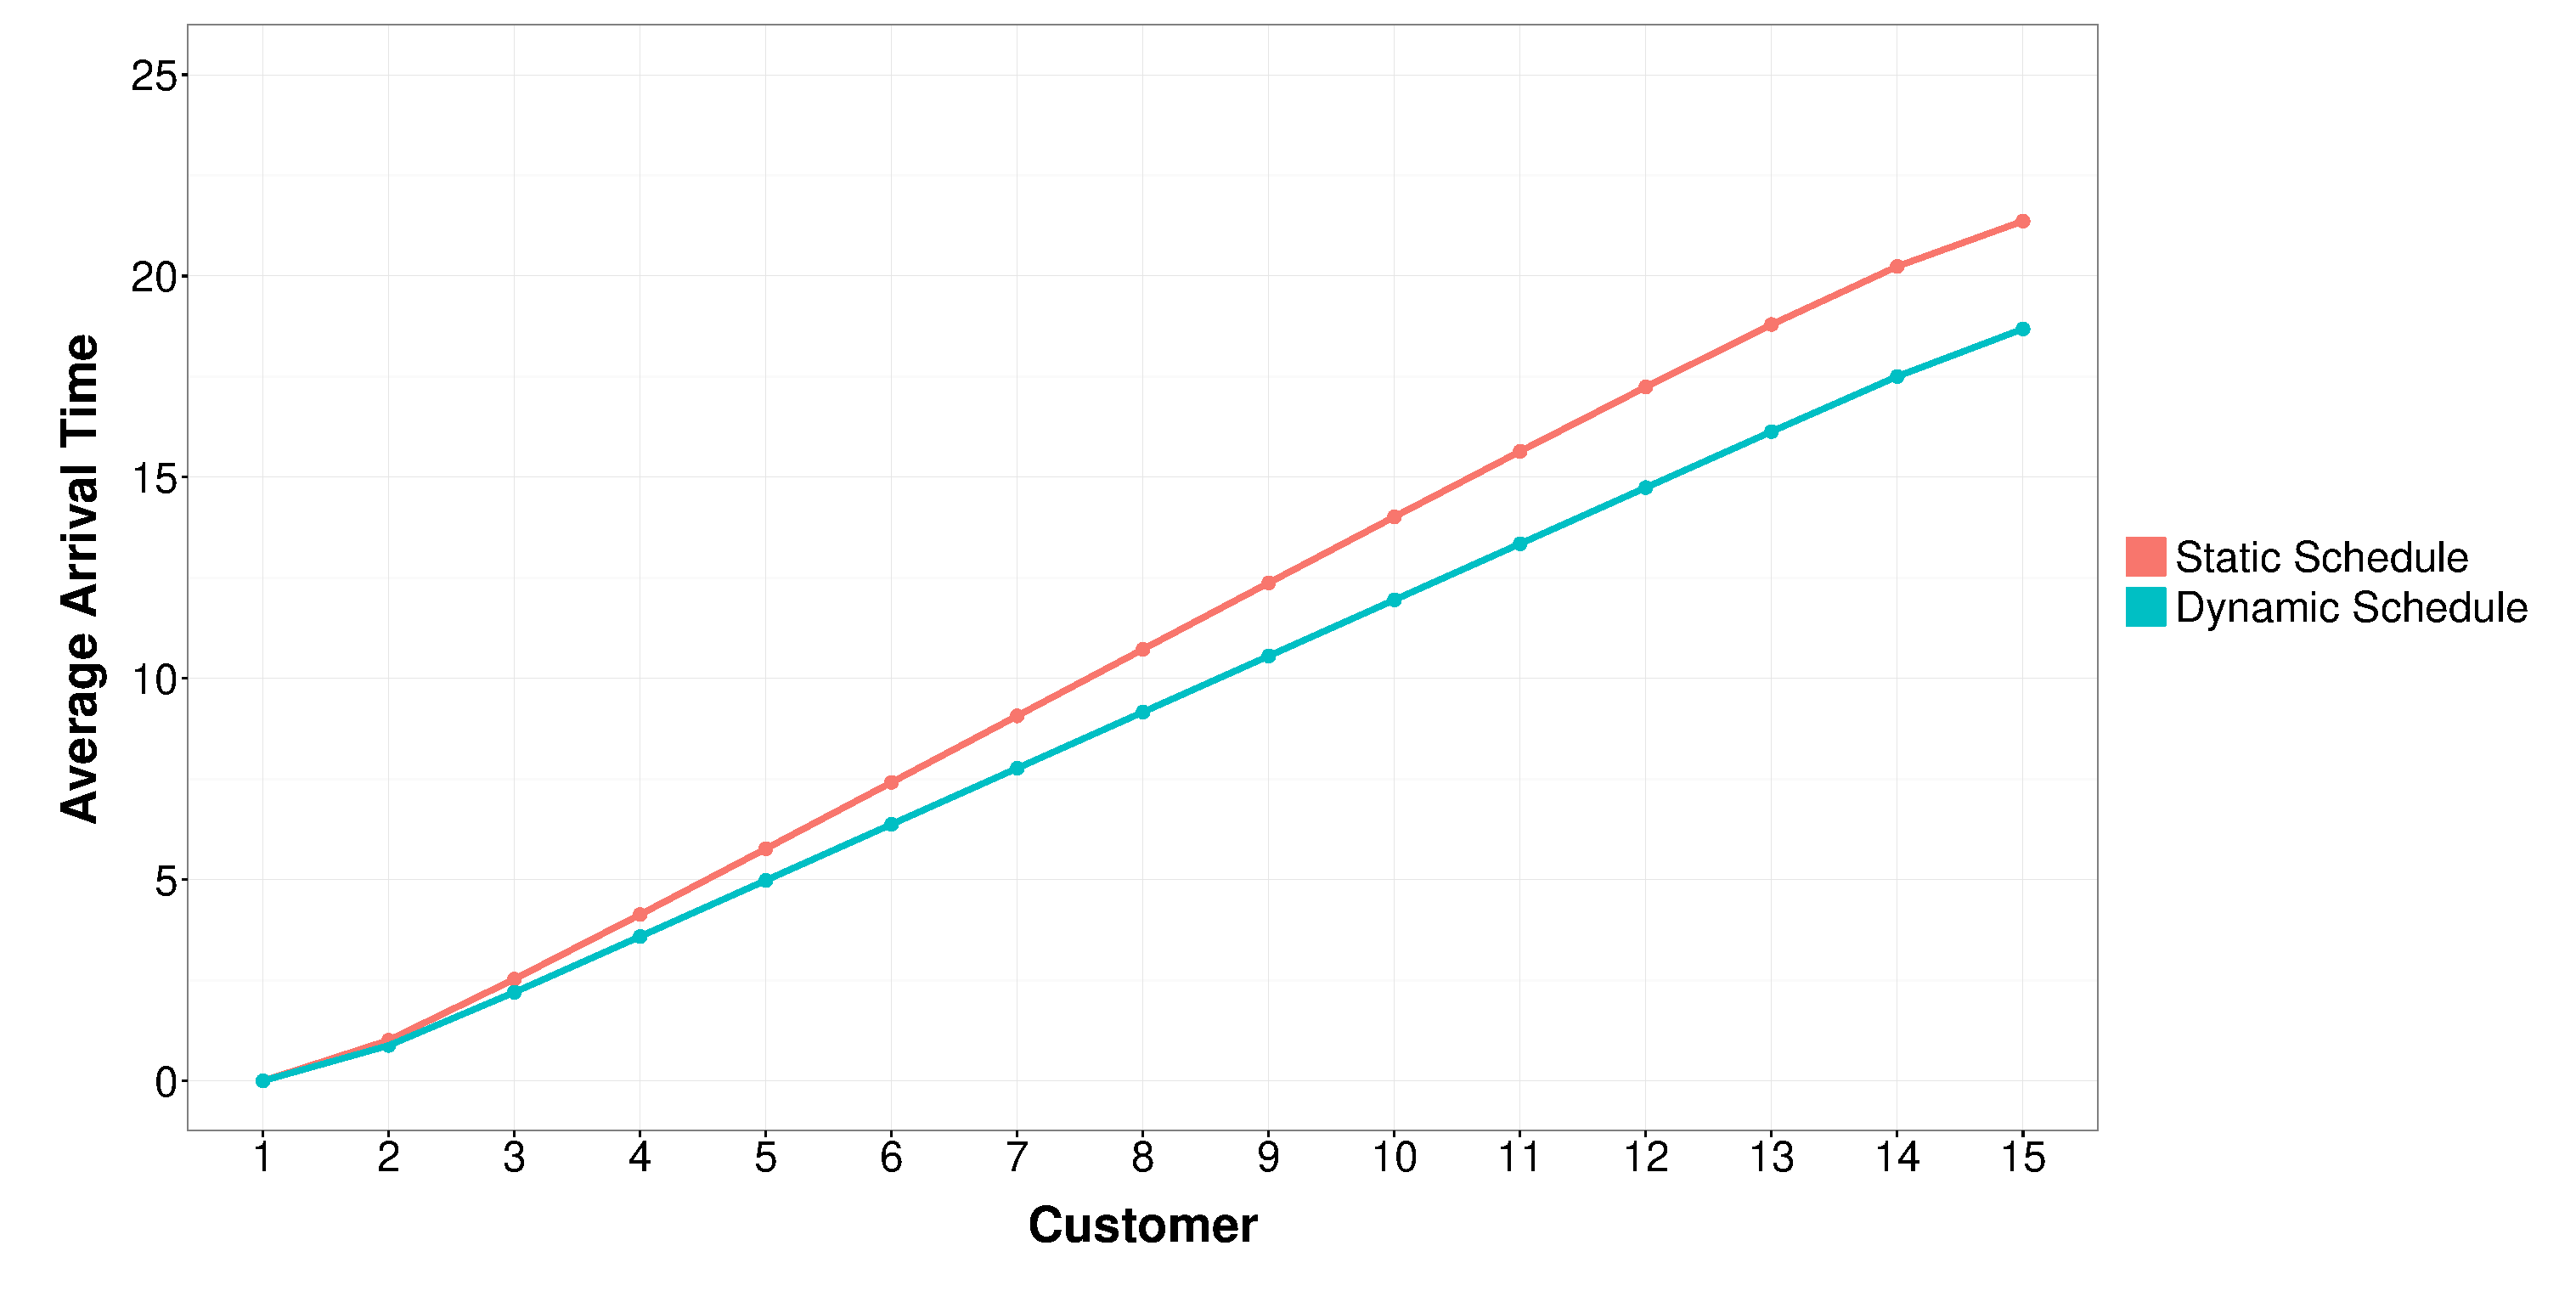
\includegraphics[width = 0.85\textwidth]{AT_Line.eps}
	\caption{Plot of the average arrival time of the $15$ customers for the static and dynamic schedules where $\mu = 1$ and $\gamma = \frac{c_{S}}{c_{S} + c_{W}} = 0.5$.}
	\label{fig:Avg_Arrival}
\end{figure}

The static schedule has fixed arrival times, whereas the arrival times are chosen progressively for the dynamic schedule. For all $15$ customers, their mean arrival time in the dynamic schedule is never later than their arrival time in the static schedule. The mean arrival times appear to be very similar for the first four or five customers. However, the later customers in the dynamic schedule appear to arrive significantly eariler than the corresponding customers in the static schedule.

\section{Customer Waiting Times}
We would expect that the earlier arrival of the customers in the dynamic schedule would lead to those customers waiting longer. This hypothesis is examined by plotting the histogram of the difference in average customer waiting time between the two schedules in Figure~\ref{fig:Diff_Wait}. As before, this is a plot of the average waiting time of the static schedule minus the average waiting time of the dynamic schedule.
\begin{figure}[htb]
	\centering
	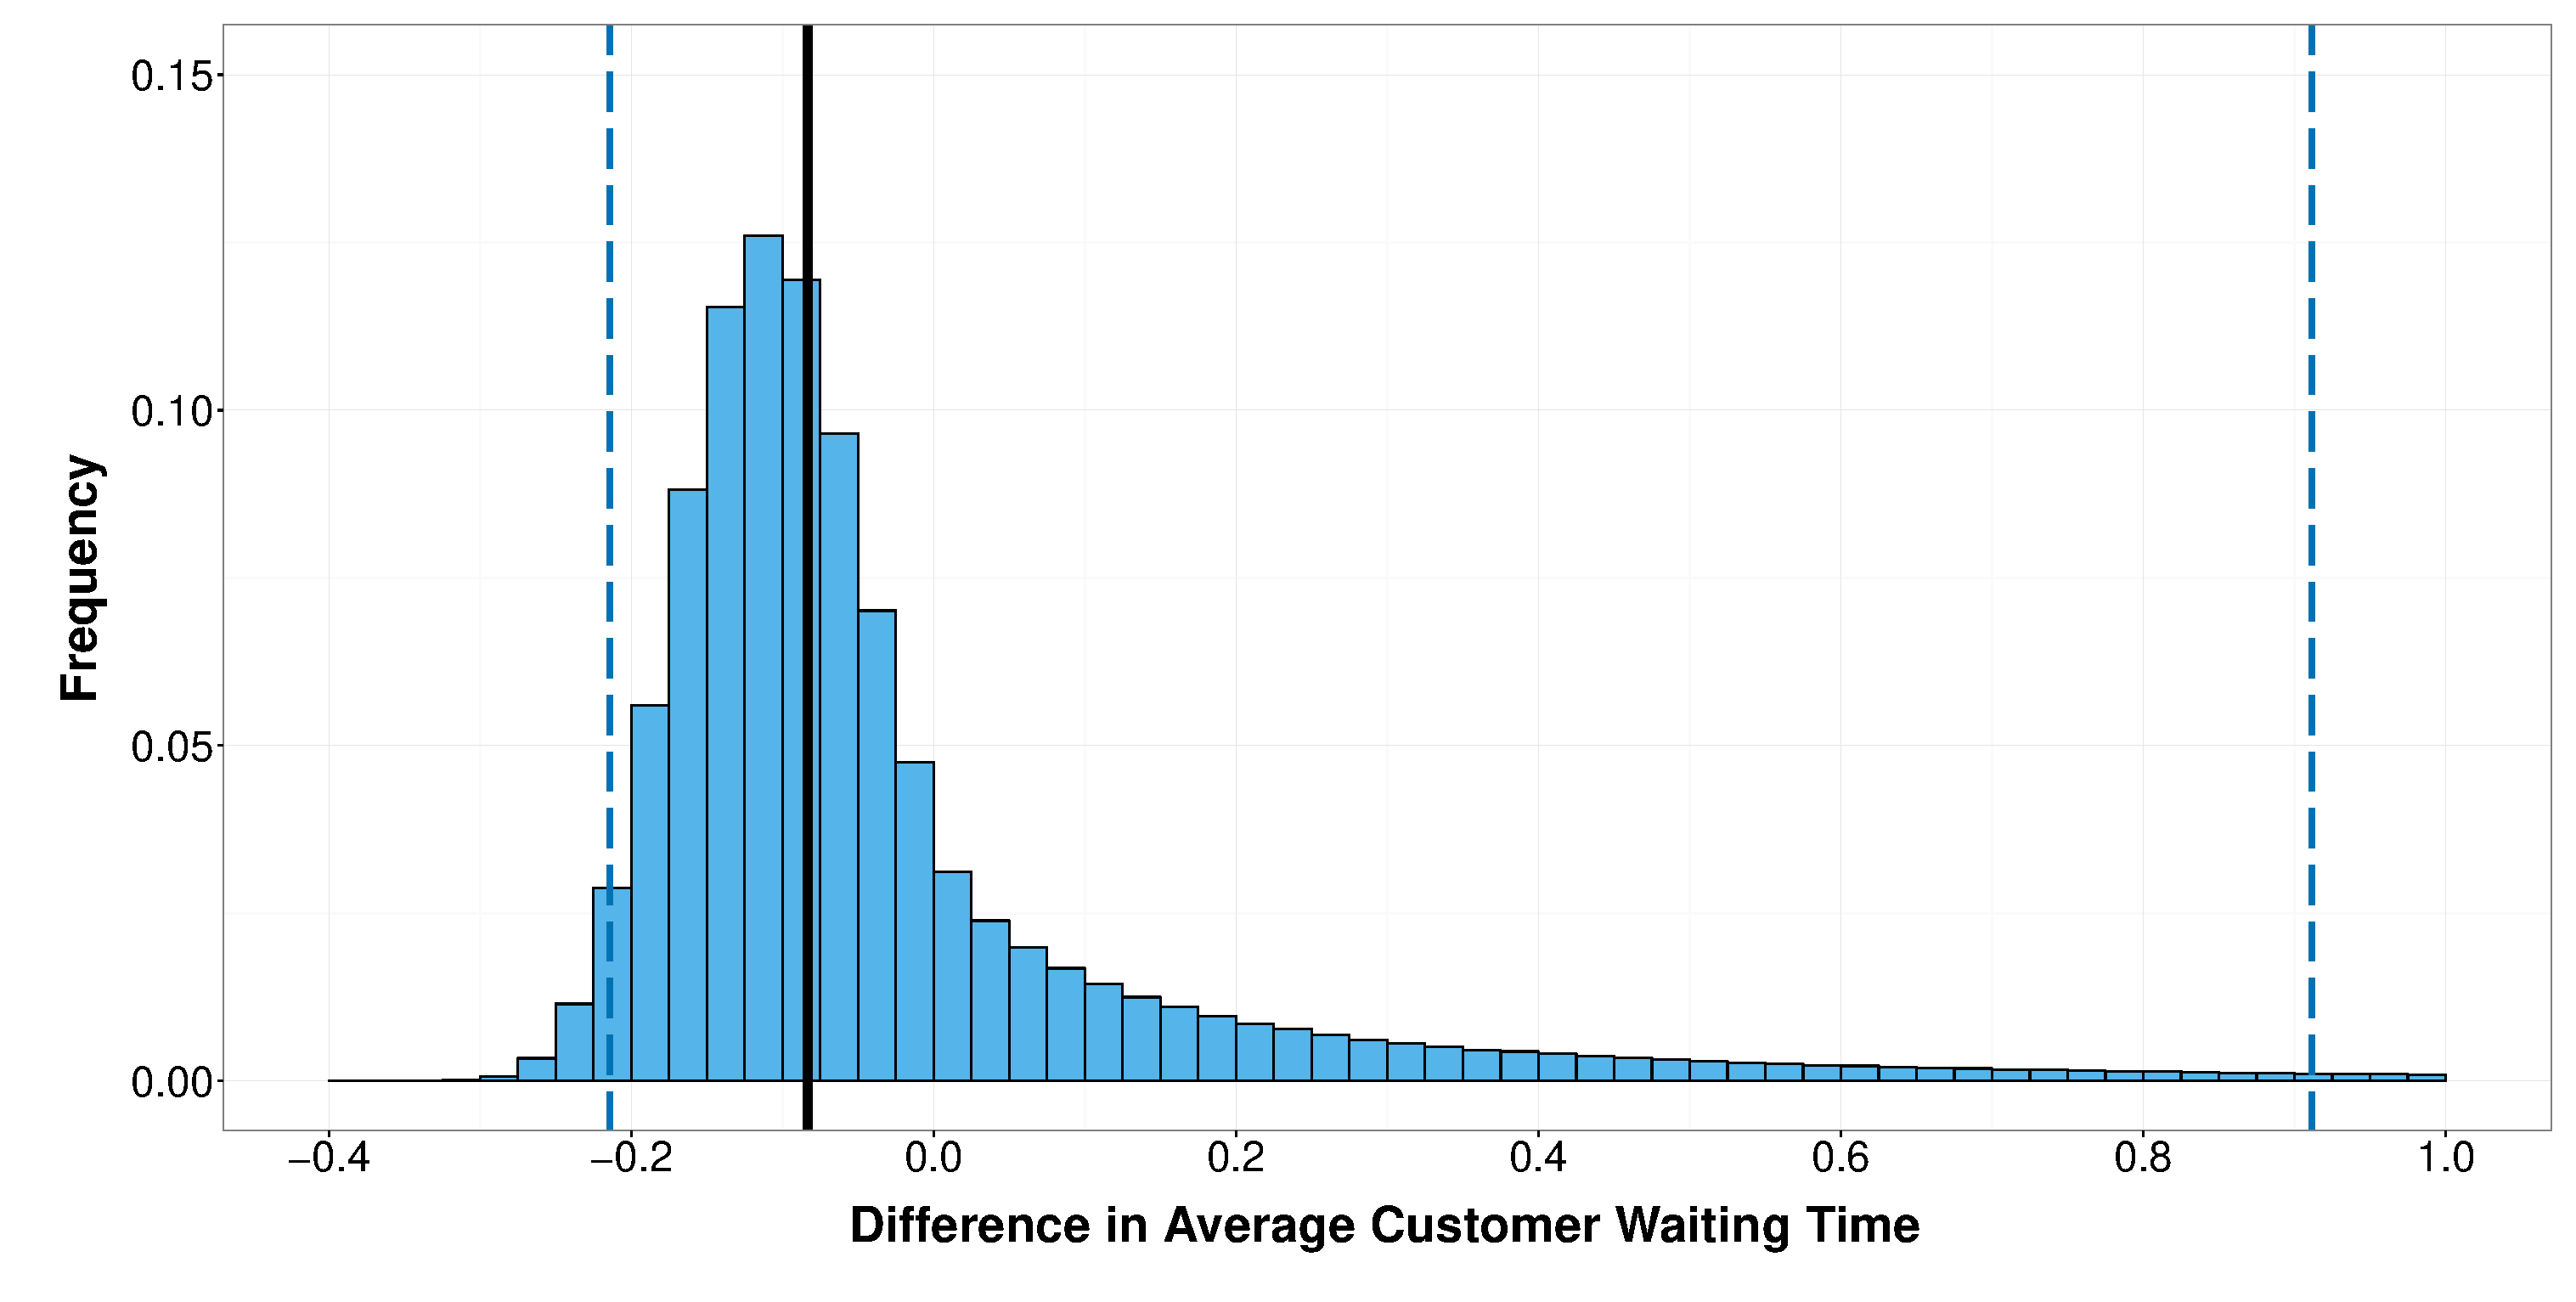
\includegraphics[width = 0.85\textwidth]{WT_Hist_Diff.eps}
	\caption{Histogram plot of the average waiting time for the static schedule minus the average waiting time for the dynamic schedule where $\mu = 1$ and $\gamma = \frac{c_{S}}{c_{S} + c_{W}} = 0.5$. The black vertical line indicates the median and the blue dashes lines indicate the upper and lower quartiles.}
	\label{fig:Diff_Wait}
\end{figure}

The $75$-th percentile of the difference in average waiting time is $0.00$. As expected, for the majority of the runs, the customers in the static schedule have a shorter average waiting time than the customers in the dynamic schedule.

However, the minimum difference in average waiting time is only $-0.33$, whereas the maximum is $8.57$. It appears that in the simulation runs where the dynamic schedule has a shorter waiting time than the static schedule, it tends to have a significantly shorter waiting time. The dynamic schedule is less prone to extremely long waiting times for the customers. This is expected behaviour as the dynamic schedule is able to react to customers having longer than expected service times and reschedule the later customers.

Another important consideration is the treatment of all the customers individually. Figure~\ref{fig:Avg_Wait_Position} plots the average waiting time of each customer individually.
\begin{figure}[htb]
	\centering
	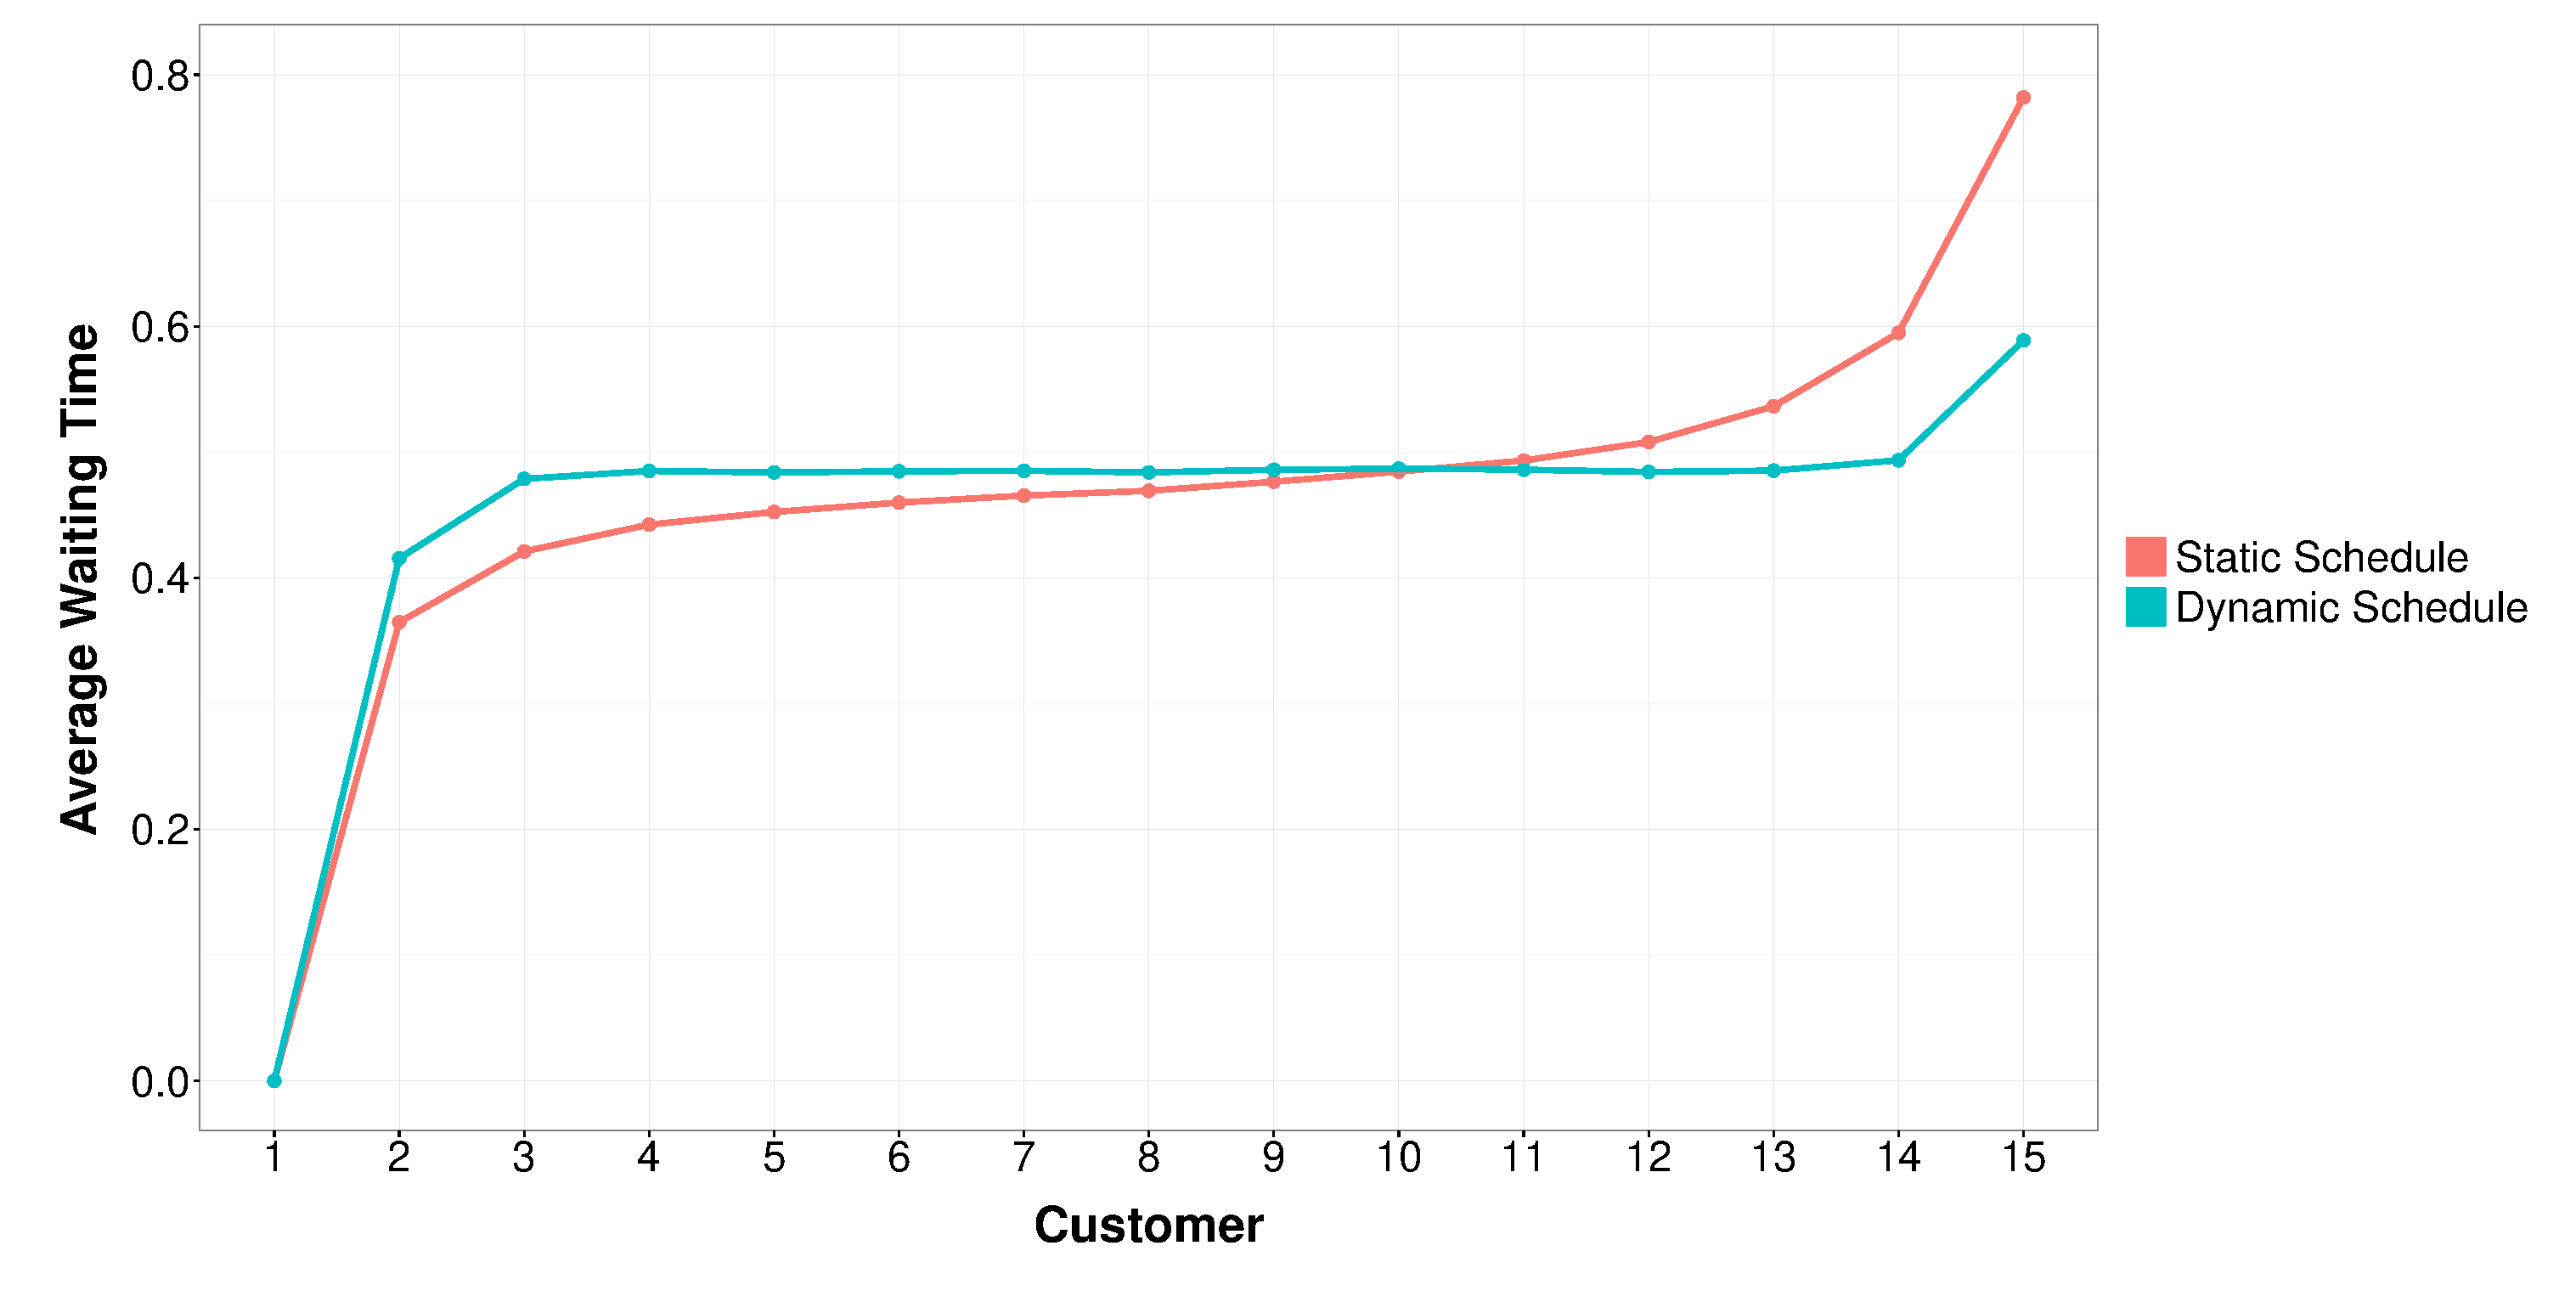
\includegraphics[width = 0.85\textwidth]{WT_Line_Avg.eps}
	\caption{Plot of the average waiting time of the $15$ customers for the static and dynamic schedules where $\mu = 1$ and $\gamma = \frac{c_{S}}{c_{S} + c_{W}} = 0.5$.}
	\label{fig:Avg_Wait_Position}
\end{figure}

In both schedules, the average waiting time of the first customer is $0$ as they are served immediately. The first few customers wait longer on average in the dynamic schedule than the static schedule. In contrast, the later few customers tend to wait significantly longer in the static schedule.

For customer $3$ to customer $14$, their average waiting times are approximately constant in the dynamic schedule, but increasing in the static schedule. It appears that the dynamic schedule is significantly `fairer' and able to spread the waiting time more evenly amongst the customers. The static schedule tends to favour the earlier customers.

Intuitively, customers prefer schedules where they are served immediately and do not have to wait. Figure~\ref{fig:No_Wait_Position} plots the proportion of runs where each customer does not have to wait.
\begin{figure}[htb]
	\centering
	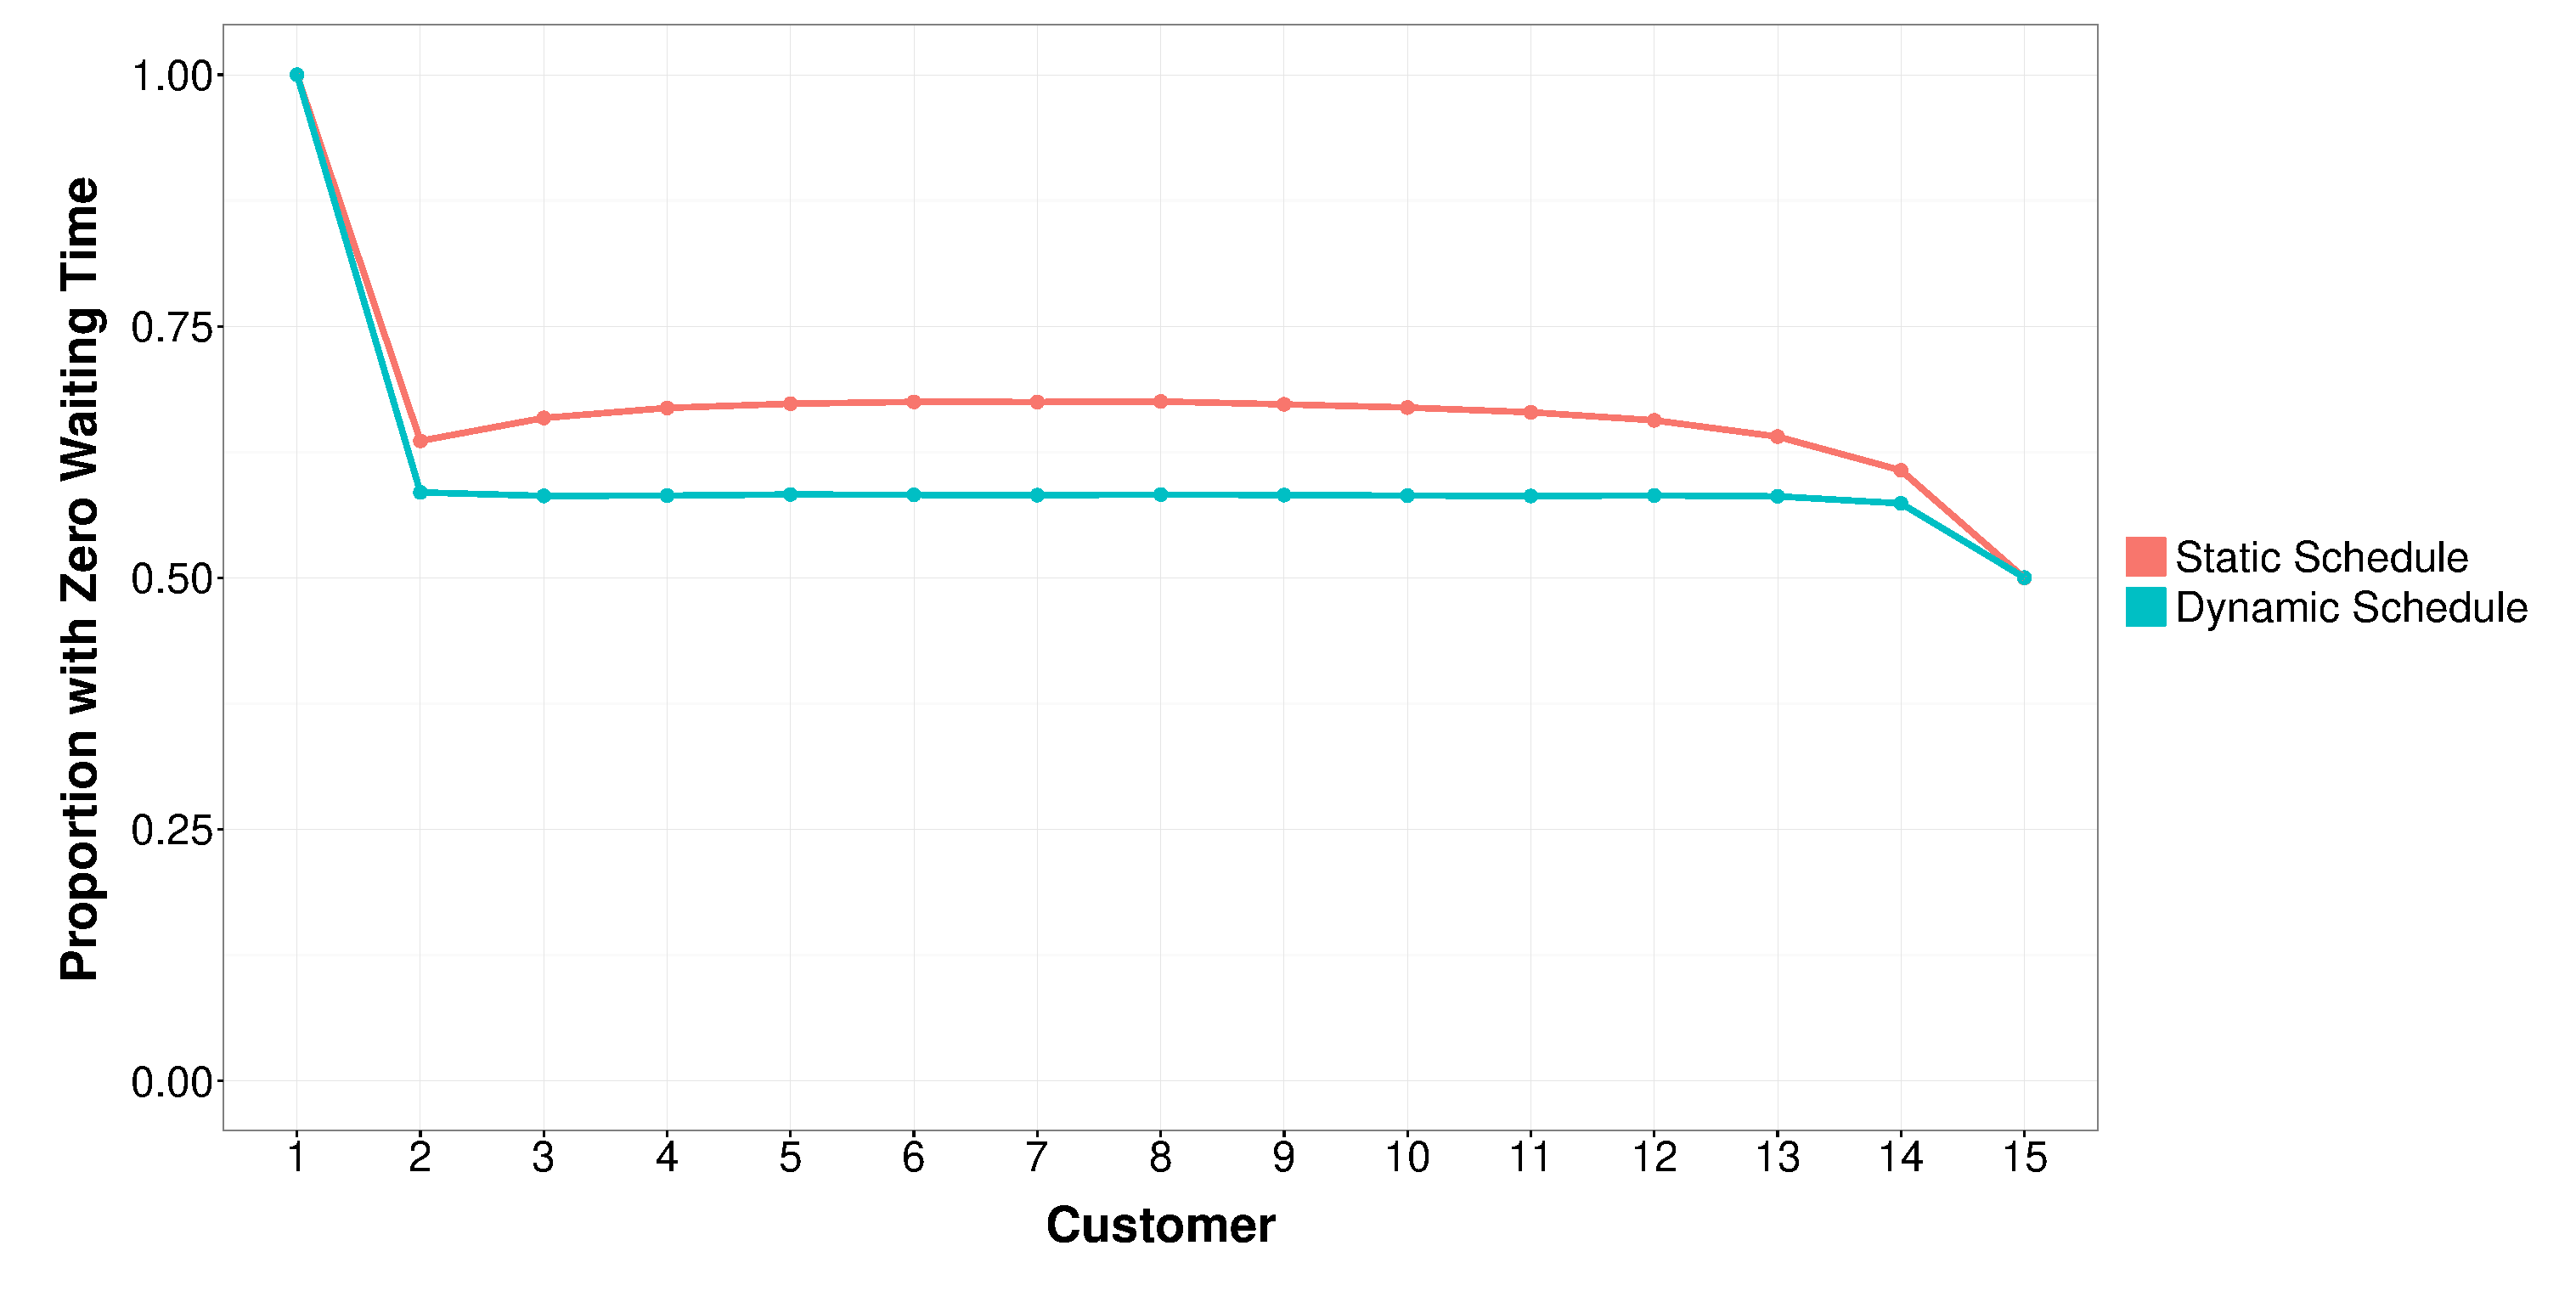
\includegraphics[width = 0.85\textwidth]{WT_Line_Prop.eps}
	\caption{Plot of the proportion of all runs where the customer does not wait for each of the $15$ customers for the static and dynamic schedules where $\mu = 1$ and $\gamma = \frac{c_{S}}{c_{S} + c_{W}} = 0.5$.}
	\label{fig:No_Wait_Position}
\end{figure}

In both schedules, the first customer never waits and is served immediately in $100 \%$ of the runs. The dynamic schedule again appears to be fairer. The proportion of runs with no waiting time appears to be constant for all except the first and last customers. This result may be provable in the general case. Future work could investigate whether a dynamic schedule always has equal probability of immediate service for all except the first and last customers.

All customers (except the first and last) are served immediately a greater proportion of the time in the static schedule than the dynamic schedule. While this is advantageous for the customers, it leads to a longer idle time of the server and thus a longer server availability time.

\section{Server Availability Time}
The schedules do not only attempt to minimise customer waiting time, but they also attempt to minimise the server availability time. Figure~\ref{fig:Two_Server} plots the histograms of the server availability times of the static and dynamic schedules for each run of the simulation.
\begin{figure}[htb]
	\centering
	\begin{subfigure}[t]{0.45\textwidth}
		\centering
		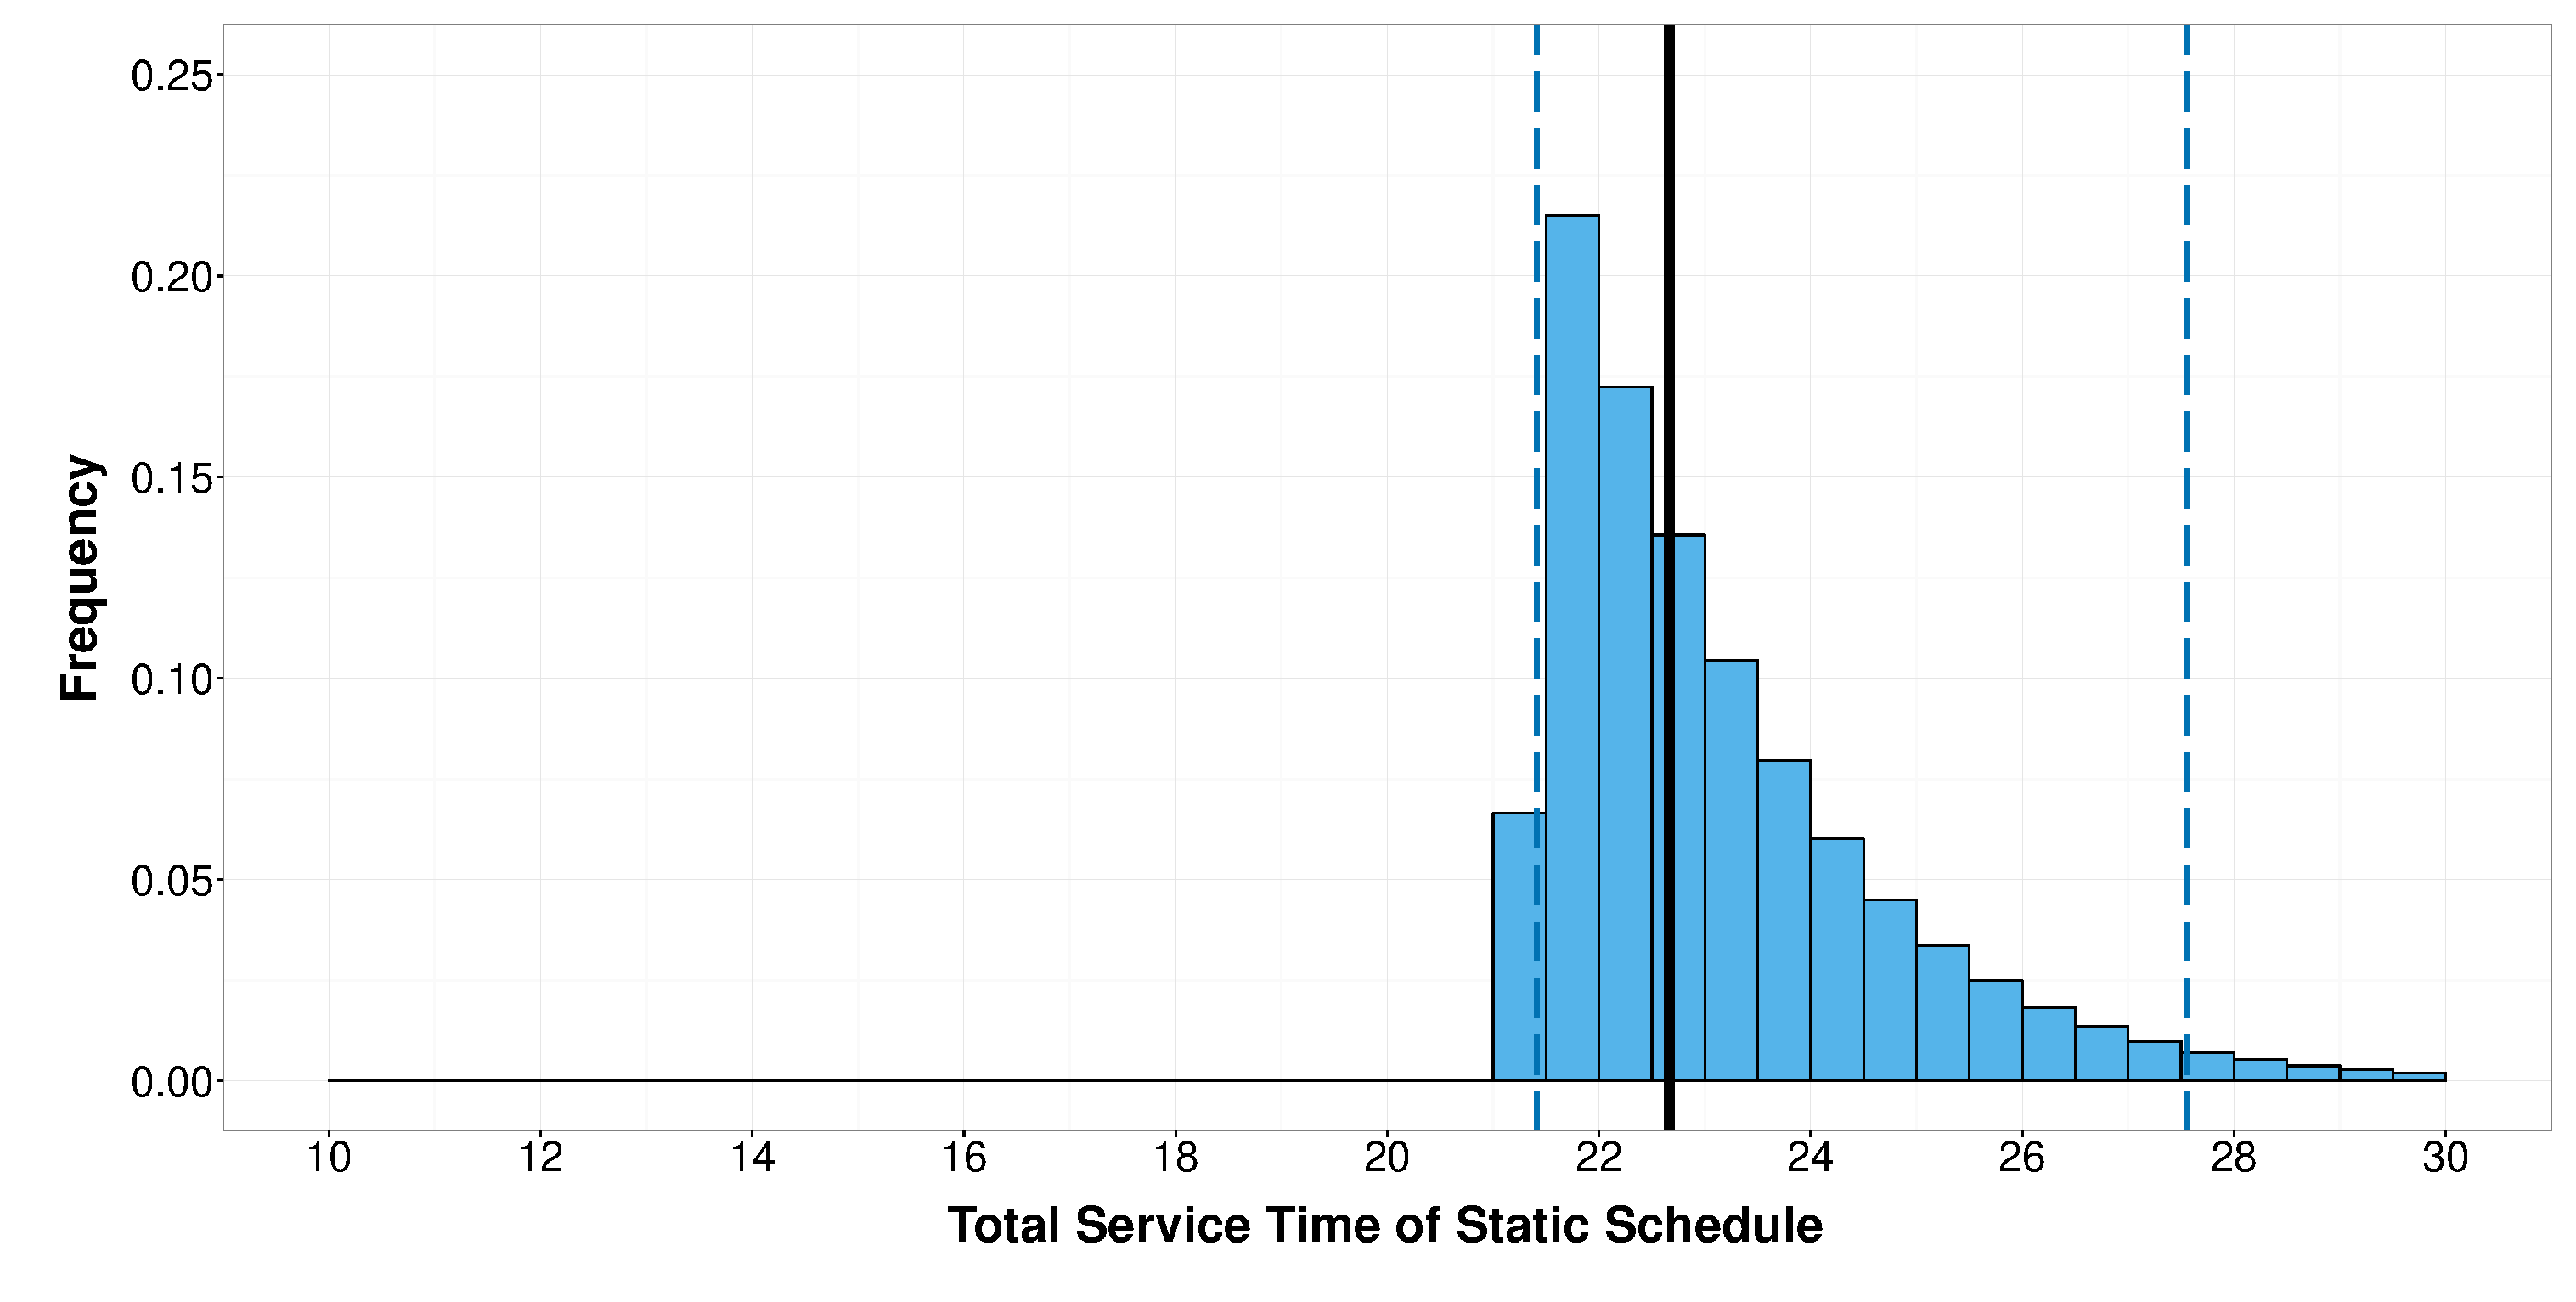
\includegraphics[width=\textwidth]{TST_Hist_Static.eps}
		\caption{}
	\end{subfigure}
	\begin{subfigure}[t]{0.45\textwidth}
		\centering
		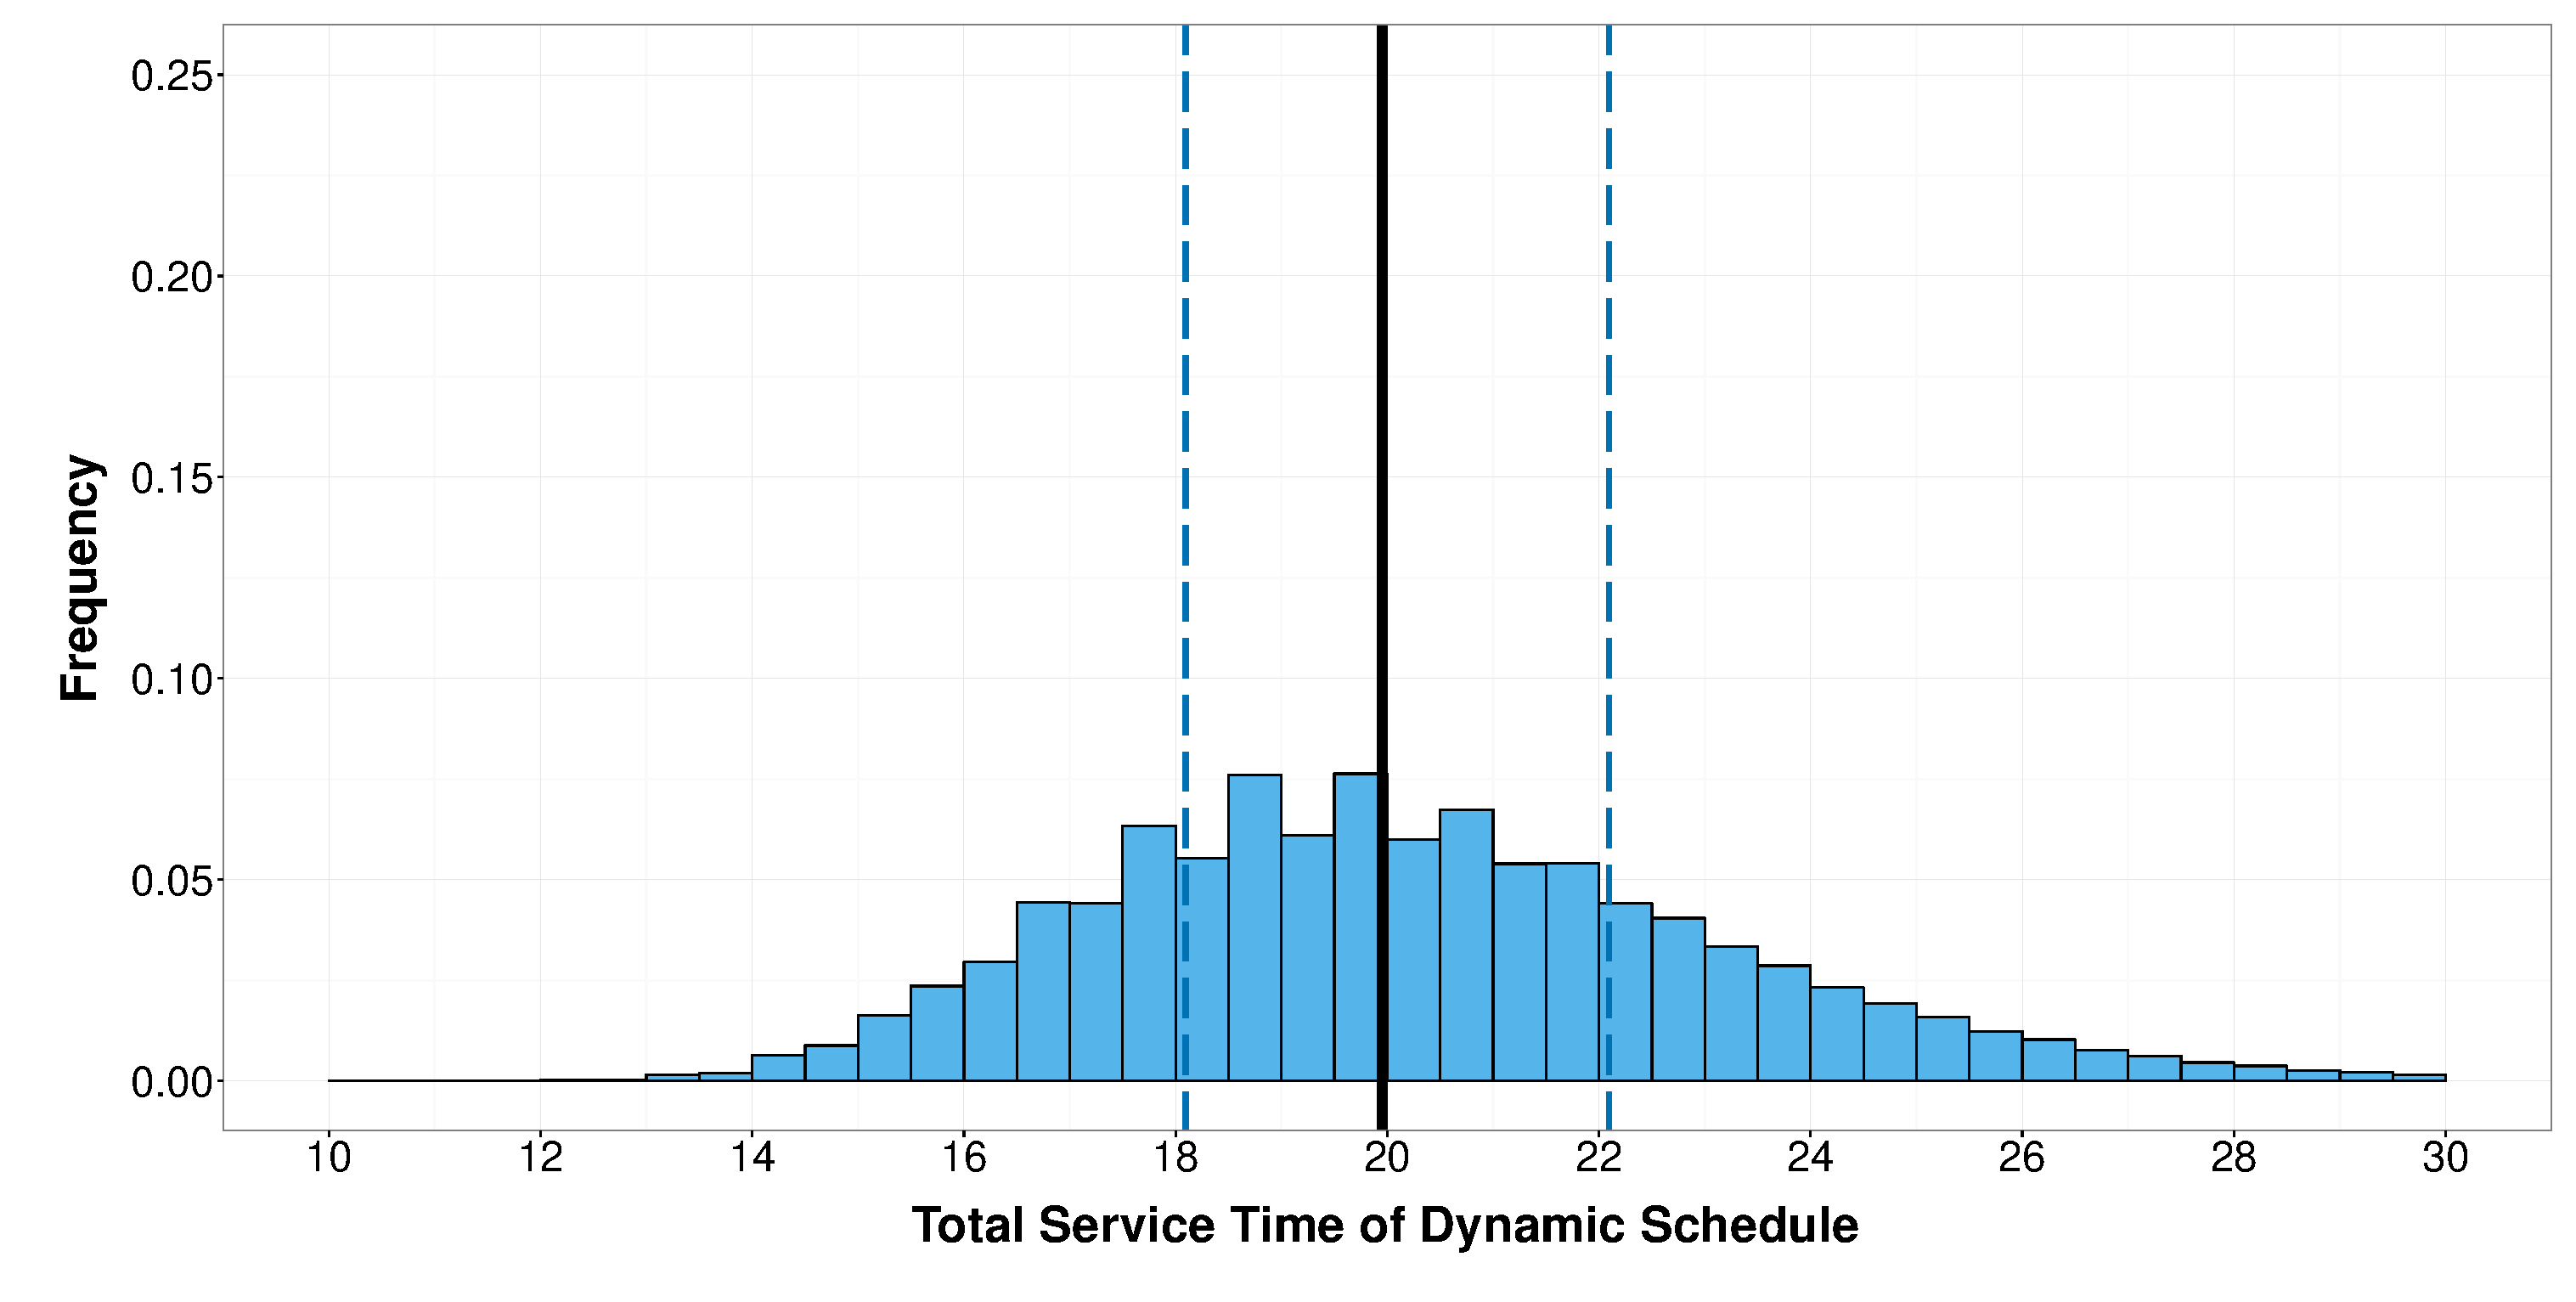
\includegraphics[width=\textwidth]{TST_Hist_Dynamic.eps}
		\caption{}
	\end{subfigure}
	\caption{Histogram plot of the server availability times for the static (a) and dynamic (b) schedules for each simulation run where $\mu = 1$ and $\gamma = \frac{c_{S}}{c_{S} + c_{W}} = 0.5$. The black vertical line indicates the median and the blue dashes lines indicate the upper and lower quartiles.}
	\label{fig:Two_Server}
\end{figure}

The median server availability time is $22.66$ for the static schedule and $19.95$ for the dynamic schedule. While the customer waiting times appear to be generally similar for both schedules, the dynamic schedule appears to attain its lower expected cost due to its lower server availability time. This agrees with the idea from Chapter~\ref{chap:Comparison} that the expected percentage cost saving is lowest where $\gamma = \frac{c_{S}}{c_{S} + c_{W}}$ is small. If the per unit time cost of the server availability time is small then the dynamic schedule's ability to reduce the server availability time is less effective at reducing the schedule cost.

Moreover, the minimum server availability time is significantly lower in the case of the dynamic schedule. The minimum server availability time is $21.37$ for the static schedule and $12.11$ for the dynamic schedule. Both minimums occur in the same run of the simulation, which is obviously a run with unusually low service times.

The static schedule is significantly limited by the fixed arrival of the last customer at $21.36$ time units. The dynamic schedule is able to adjust the customer arrival times and attain a broader range of server availability times that are lower on average.